\documentclass[hyperref,]{ctexart}
\usepackage{lmodern}
\usepackage{amssymb,amsmath}
\usepackage{ifxetex,ifluatex}
\usepackage{fixltx2e} % provides \textsubscript
\ifnum 0\ifxetex 1\fi\ifluatex 1\fi=0 % if pdftex
  \usepackage[T1]{fontenc}
  \usepackage[utf8]{inputenc}
\else % if luatex or xelatex
  \ifxetex
    \usepackage{xltxtra,xunicode}
  \else
    \usepackage{fontspec}
  \fi
  \defaultfontfeatures{Mapping=tex-text,Scale=MatchLowercase}
  \newcommand{\euro}{€}
\fi
% use upquote if available, for straight quotes in verbatim environments
\IfFileExists{upquote.sty}{\usepackage{upquote}}{}
% use microtype if available
\IfFileExists{microtype.sty}{%
\usepackage{microtype}
\UseMicrotypeSet[protrusion]{basicmath} % disable protrusion for tt fonts
}{}
\ifxetex
  \usepackage[setpagesize=false, % page size defined by xetex
              unicode=false, % unicode breaks when used with xetex
              xetex]{hyperref}
\else
  \usepackage[unicode=true]{hyperref}
\fi
\usepackage[usenames,dvipsnames]{color}
\hypersetup{breaklinks=true,
            bookmarks=true,
            pdfauthor={蓝海; 彭莉},
            pdftitle={分析朱志权-技术报告},
            colorlinks=true,
            citecolor=blue,
            urlcolor=blue,
            linkcolor=magenta,
            pdfborder={0 0 0}}
\urlstyle{same}  % don't use monospace font for urls
\usepackage{longtable,booktabs}
\usepackage{graphicx,grffile}
\makeatletter
\def\maxwidth{\ifdim\Gin@nat@width>\linewidth\linewidth\else\Gin@nat@width\fi}
\def\maxheight{\ifdim\Gin@nat@height>\textheight\textheight\else\Gin@nat@height\fi}
\makeatother
% Scale images if necessary, so that they will not overflow the page
% margins by default, and it is still possible to overwrite the defaults
% using explicit options in \includegraphics[width, height, ...]{}
\setkeys{Gin}{width=\maxwidth,height=\maxheight,keepaspectratio}
\setlength{\emergencystretch}{3em}  % prevent overfull lines
\providecommand{\tightlist}{%
  \setlength{\itemsep}{0pt}\setlength{\parskip}{0pt}}
\setcounter{secnumdepth}{5}

\title{分析朱志权-技术报告}
\author{蓝海 \and 彭莉}
\date{}

% Redefines (sub)paragraphs to behave more like sections
\ifx\paragraph\undefined\else
\let\oldparagraph\paragraph
\renewcommand{\paragraph}[1]{\oldparagraph{#1}\mbox{}}
\fi
\ifx\subparagraph\undefined\else
\let\oldsubparagraph\subparagraph
\renewcommand{\subparagraph}[1]{\oldsubparagraph{#1}\mbox{}}
\fi

\begin{document}
\maketitle

{
\setcounter{tocdepth}{2}
\tableofcontents
}
\section{业绩表现}

\subsection{朱志权}

朱志权:经济学学士。具有基金从业资格。基金投资部总监兼投资总监。曾任职于中信证券上海总部、长盛基金管理有限公司、富国基金管理有限公司、中海信托管理有限公司、银河基金管理有限公司。2008年6月加入泰信基金管理有限公司,2008年6月28日至2012年3月1日担任泰信优质生活股票基金基金经理;自2012年3月1日至2015年2月5日任泰信先行策略开放式证券投资基金基金经理;2010年1月16日至今担任泰信优势增长混合基金基金经理。

朱志权前后共管理过4个混合型的的公墓基金产品,其中泰信智选成长混合基金创设时间太短,不具备分析价值,所以我们重点的挑选了3只基金为代表进行分析。它们是泰信先行策略、泰信优势增长和泰信优质生活混合。

\subsection{业绩表现}\label{-1}

泰信智选成长混合和泰信优质生活混合是朱志权在当前正在管理的产品,其业绩标准虽然不尽相同,但是沪深300依旧是重要的比较基准。
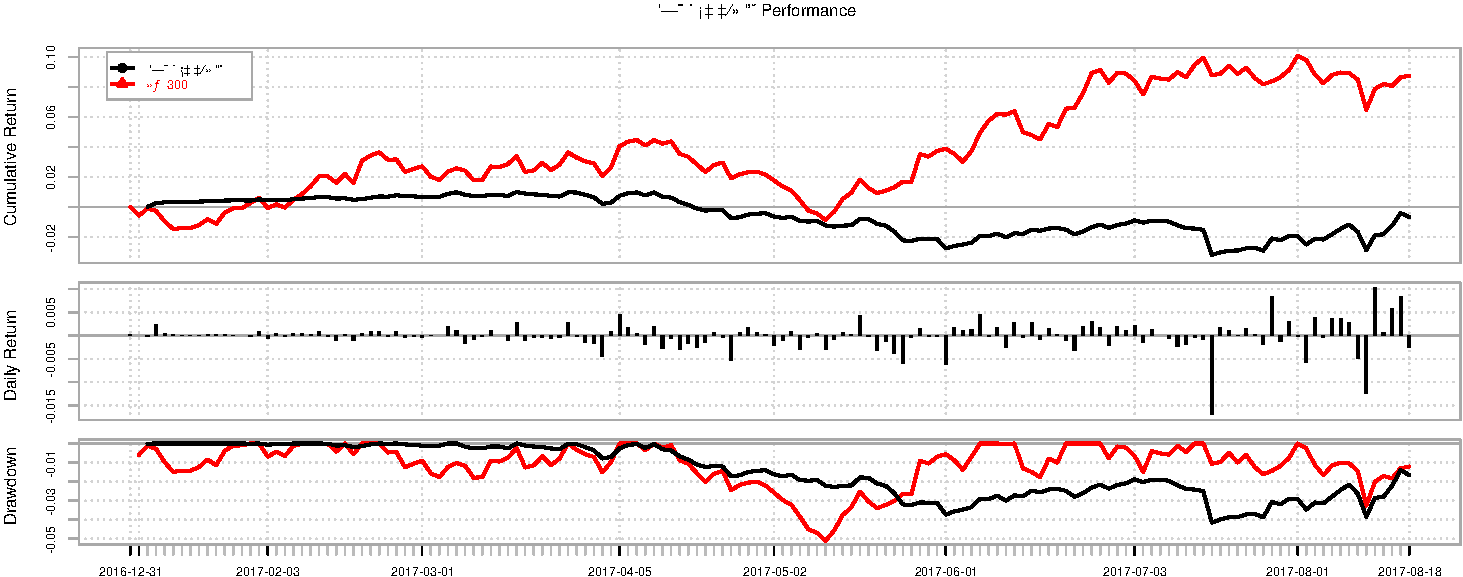
\includegraphics{zzq-detail_files/figure-latex/unnamed-chunk-2-1.pdf}

\begin{longtable}[]{@{}llclc@{}}
\toprule
名称 & 最后半年 & 夏普率 & 一年 & 夏普率\tabularnewline
\midrule
\endhead
泰信智选成长混合 & -1.3\% & -1.1 & -0.67\% & -1.1\tabularnewline
沪深300 & 6.6\% & 1.0 & 9.18\% & 1.2\tabularnewline
\bottomrule
\end{longtable}

泰信优势增长与沪深300比较:

\begin{figure}[htbp]
\centering
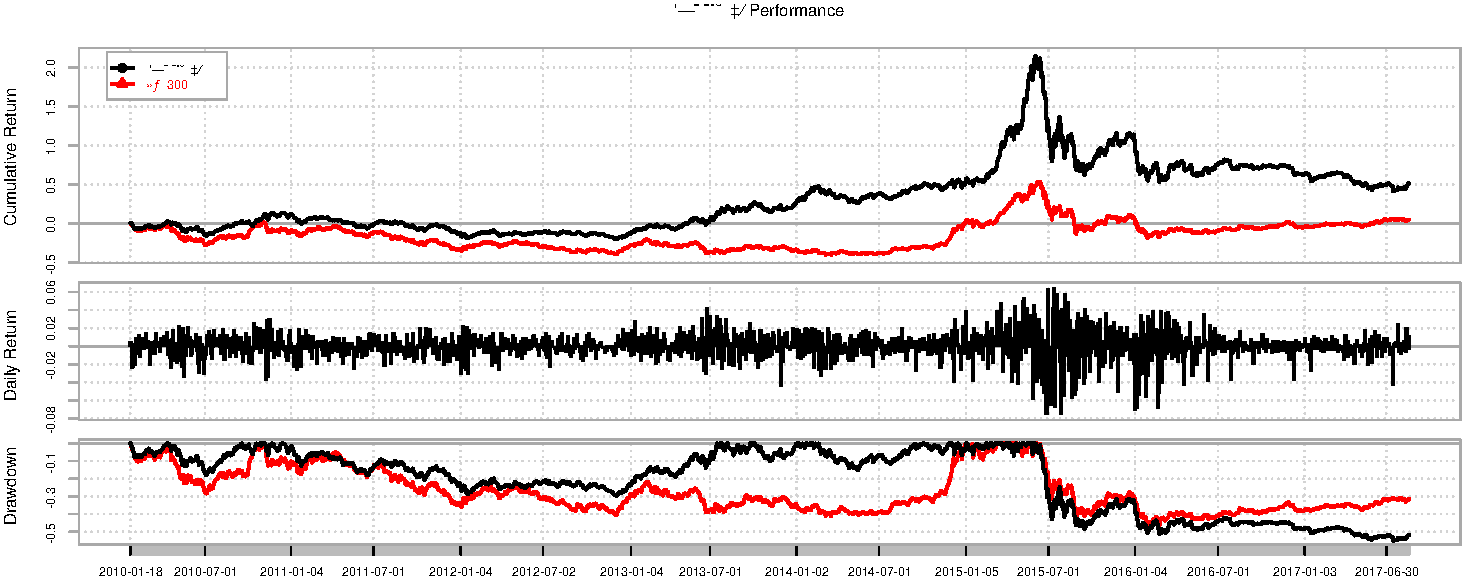
\includegraphics{zzq-detail_files/figure-latex/unnamed-chunk-3-1.pdf}
\caption{基金累计回报率与回撤}
\end{figure}

\begin{longtable}[]{@{}llclclclc@{}}
\toprule
名称 & 最后半年 & 夏普率 & 一年 & 夏普率 & 两年 & 夏普率 & 三年 &
夏普率\tabularnewline
\midrule
\endhead
泰信优势增长 & -6.1\% & -1.1 & -11\% & -1.1 & -31\% & -0.69 & 10\% &
-0.02\tabularnewline
沪深300 & 6.6\% & 1.0 & 15\% & 1.1 & -12\% & -0.35 & 68\% &
0.52\tabularnewline
\bottomrule
\end{longtable}

2015年股灾之前大多数时候该基金的业绩跑过沪深300,股灾之后的表现基本低于沪深300。朱志权自身认为投资成长股,能够获取翻倍的业绩表现才是投资的乐趣所在,而2015年股灾以后的风格是一些大盘价值和近期的周期股的表现时刻,虽然也能挣钱,但是最多的投资收益不会超过100\%。与其费心费力的去追随这样的风潮,不如修养身心,准备迎接今年年底或者明年的成长股的新风潮。\footnote{坚持自己的投资风格(价值体系)是投资人应有的素质,但是在坚持和固执之间并没有明确的分界线。}

同时我们以沪深300作为市场组合,计算该基金的CAPM模型,得到如下结果。

\begin{longtable}[]{@{}lc@{}}
\toprule
& 泰信优势增长 to 沪深300\tabularnewline
\midrule
\endhead
Alpha & 0.00\tabularnewline
Beta & 0.69\tabularnewline
Beta+ & 0.58\tabularnewline
Beta- & 0.78\tabularnewline
R-squared & 0.51\tabularnewline
Annualized Alpha & 0.06\tabularnewline
Correlation & 0.71\tabularnewline
Correlation p-value & 0.00\tabularnewline
Tracking Error & 0.18\tabularnewline
Active Premium & 0.05\tabularnewline
Information Ratio & 0.28\tabularnewline
Treynor Ratio & 0.08\tabularnewline
\bottomrule
\end{longtable}

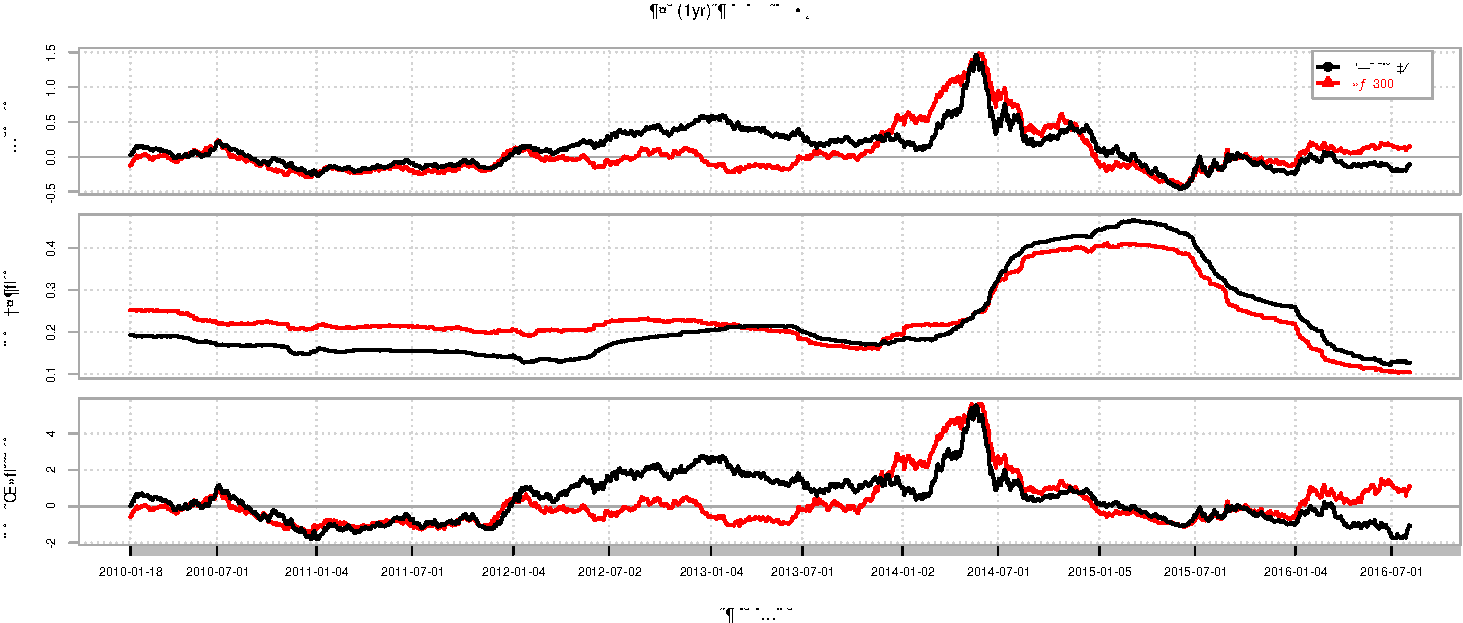
\includegraphics{zzq-detail_files/figure-latex/unnamed-chunk-5-1.pdf}
在2014之前,投资泰信优势增长一年能够获得比沪深300指数更好的收益,尤其是2012年道2014之间超额收益显著\footnote{这指的的投资起始时间。}。但是在之后,投资该基金就不如投资沪深300指数划算了。

\subsection{历史表现}

\subsubsection{泰信先行策略}

朱志权的管理该基金期间同时也管理了泰信优势增长,所以我们可以看到其业绩表现上的高度相似性。

\begin{figure}[htbp]
\centering
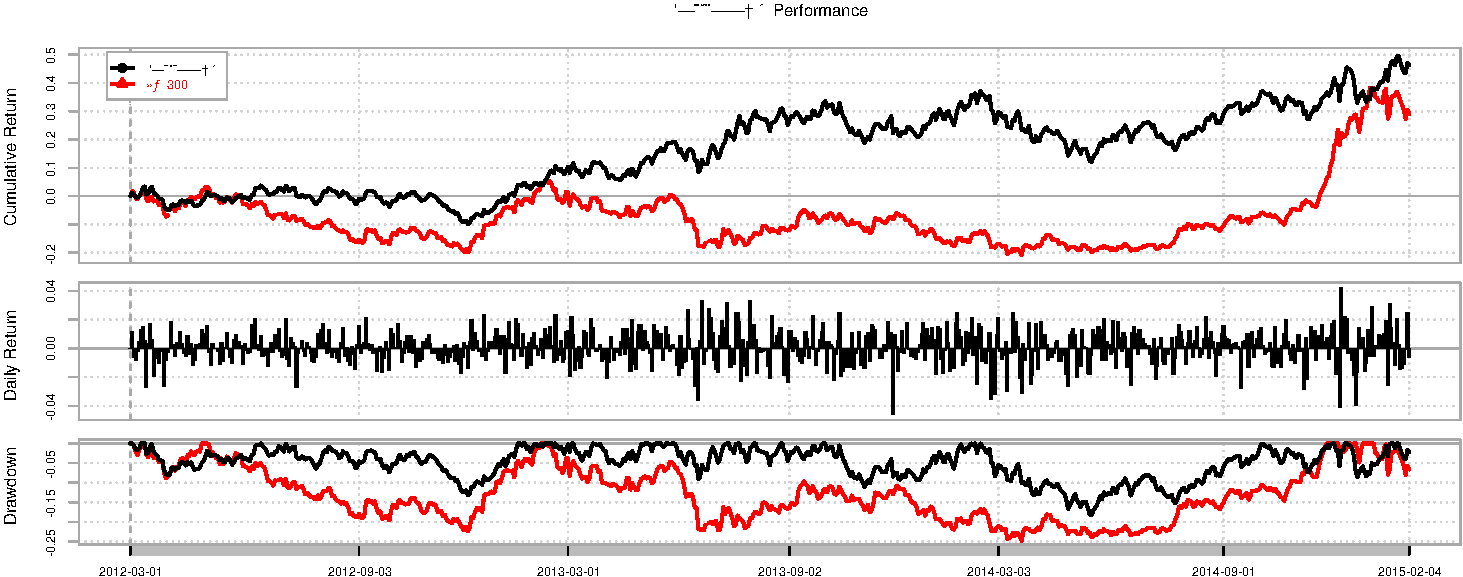
\includegraphics{zzq-detail_files/figure-latex/unnamed-chunk-6-1.pdf}
\caption{基金累计回报率与回撤}
\end{figure}

\begin{longtable}[]{@{}llclclclc@{}}
\toprule
名称 & 最后半年 & 夏普率 & 一年 & 夏普率 & 两年 & 夏普率 & 三年 &
夏普率\tabularnewline
\midrule
\endhead
泰信先行策略 & 20\% & 1.9 & 15\% & 0.53 & 48\% & 0.90 & 46\% &
0.52\tabularnewline
沪深300 & 46\% & 4.1 & 56\% & 2.31 & 37\% & 0.64 & 29\% &
0.25\tabularnewline
\bottomrule
\end{longtable}

\begin{figure}[htbp]
\centering
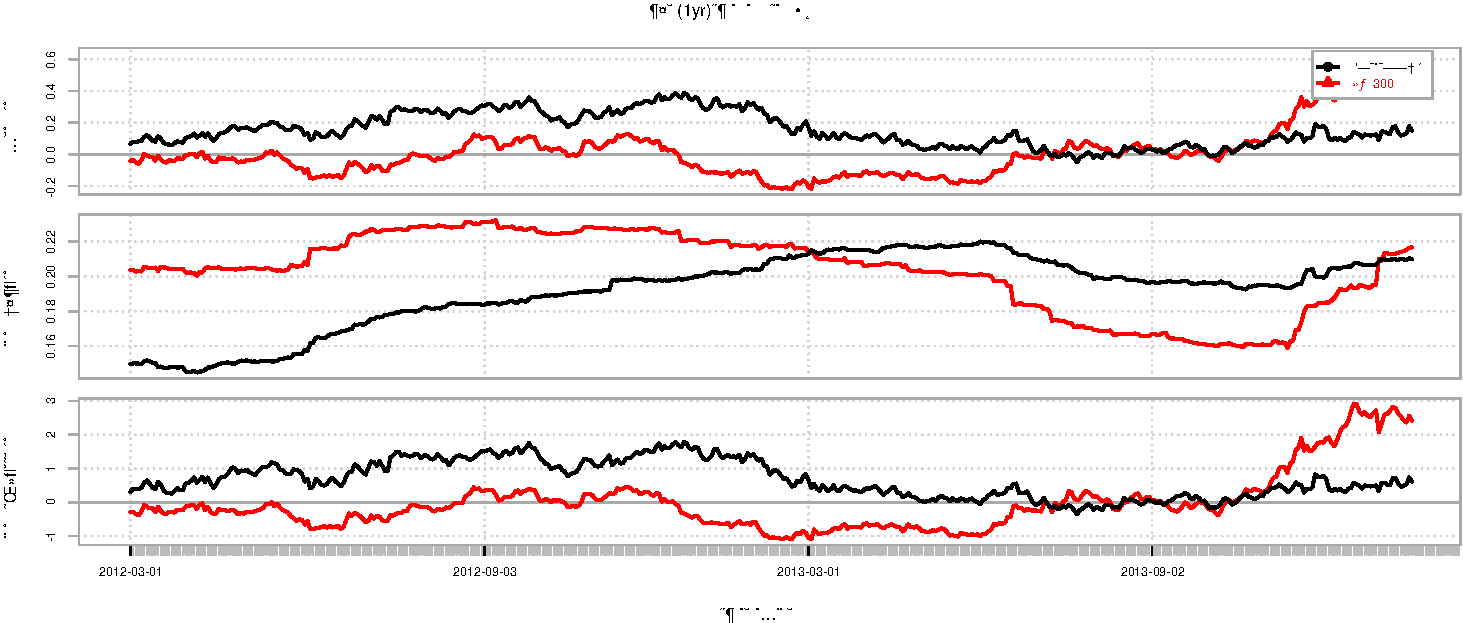
\includegraphics{zzq-detail_files/figure-latex/unnamed-chunk-7-1.pdf}
\caption{投资者收益风险比较}
\end{figure}

\subsubsection{泰信优质生活混合}

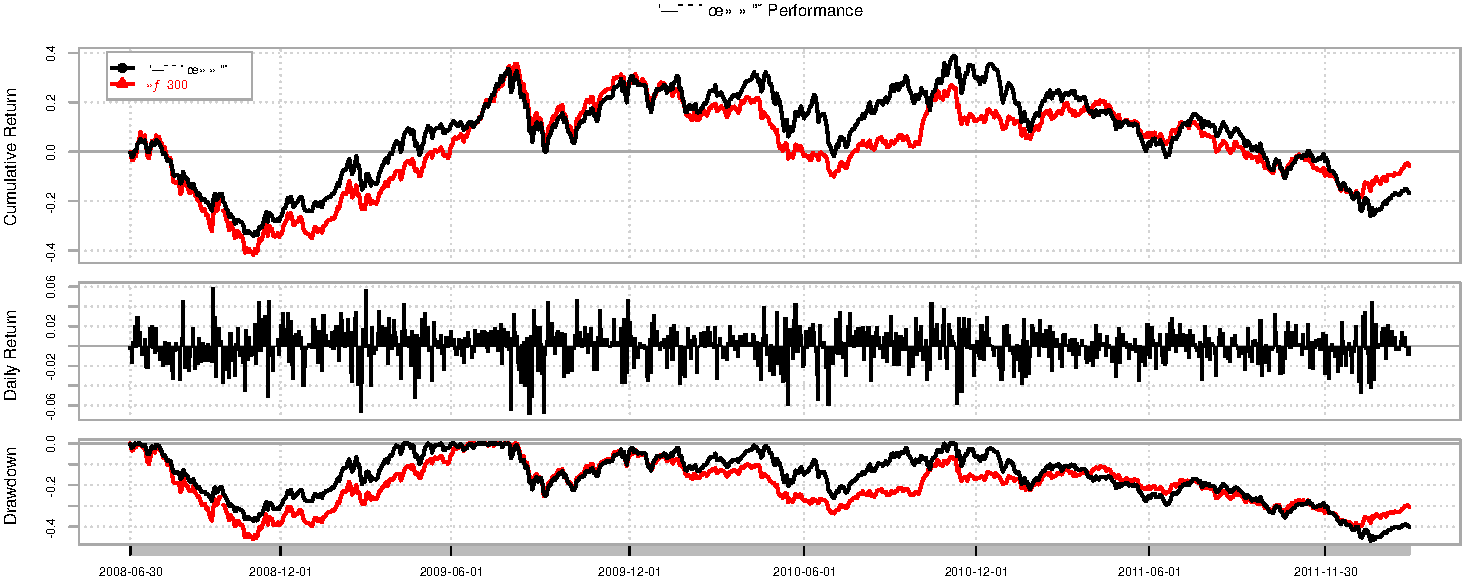
\includegraphics{zzq-detail_files/figure-latex/unnamed-chunk-8-1.pdf}

\begin{longtable}[]{@{}llclclclc@{}}
\toprule
名称 & 最后半年 & 夏普率 & 一年 & 夏普率 & 两年 & 夏普率 & 三年 &
夏普率\tabularnewline
\midrule
\endhead
泰信优质生活混合 & -23.3\% & -1.64 & -32\% & -1.4 & -32\% & -0.72 &
4.9\% & -0.08\tabularnewline
沪深300 & -7.1\% & -0.69 & -19\% & -1.0 & -22\% & -0.59 & 37.3\% &
0.26\tabularnewline
\bottomrule
\end{longtable}

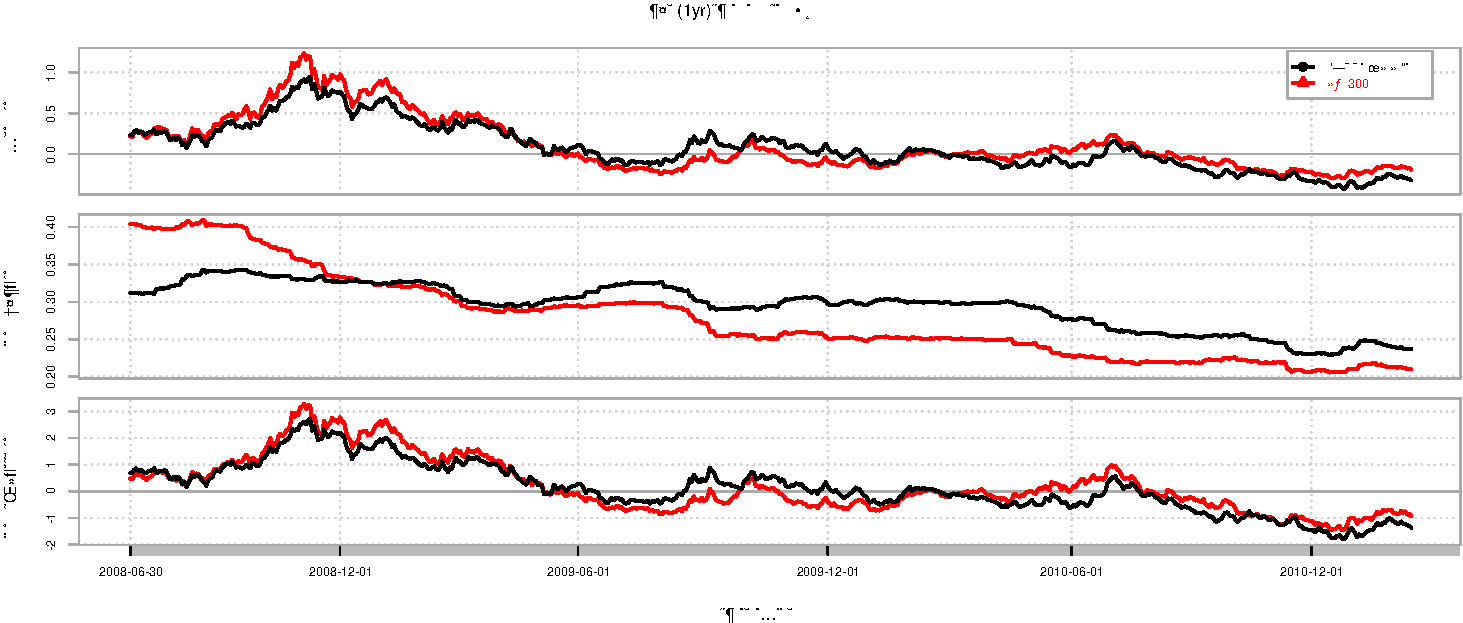
\includegraphics{zzq-detail_files/figure-latex/unnamed-chunk-8-2.pdf}

总的来说,在成长股风行的相当一段时间,朱志权完成了很亮眼的业绩报告。但是在2015年股灾之后的表现,则差强人意。

\section{风格分析}

\subsection{交易风格:低换手、高PE}\label{pe}

当前管理的泰信优势增长展现的风格数据为:

\begin{longtable}[]{@{}lcccccc@{}}
\toprule
日期 & 换手率 & 排名\% & 持有期 & 排名\% & 前十占比\% &
排名\%\tabularnewline
\midrule
\endhead
2010 Q2 & 179 & 47 & 0.29 & 54 & 42 & 64\tabularnewline
2010 Q4 & 418 & 38 & 0.14 & 60 & 38 & 87\tabularnewline
2011 Q2 & 120 & 59 & 0.44 & 42 & 42 & 67\tabularnewline
2011 Q4 & 285 & 47 & 0.20 & 60 & 41 & 83\tabularnewline
2012 Q2 & 156 & 50 & 0.33 & 60 & 45 & 73\tabularnewline
2012 Q4 & 258 & 56 & 0.22 & 54 & 39 & 87\tabularnewline
2013 Q2 & 140 & 66 & 0.36 & 36 & 46 & 81\tabularnewline
2013 Q4 & 210 & 78 & 0.23 & 35 & 46 & 79\tabularnewline
2014 Q2 & 69 & 88 & 0.78 & 8 & 44 & 73\tabularnewline
2014 Q4 & 301 & 67 & 0.17 & 46 & 56 & 48\tabularnewline
2015 Q2 & 181 & 78 & 0.31 & 17 & 56 & 60\tabularnewline
2015 Q4 & 292 & 92 & 0.27 & 16 & 42 & 70\tabularnewline
2016 Q2 & 42 & 100 & 1.25 & 7 & 33 & 83\tabularnewline
2016 Q4 & 93 & 100 & 0.56 & 10 & 31 & 86\tabularnewline
\bottomrule
\end{longtable}

\begin{longtable}[]{@{}lccccrcrc@{}}
\toprule
日期 & 行业前5占比\% & 排名\% & 平均集中度 & 排名\% & PE & 排名\% & PB &
排名\%\tabularnewline
\midrule
\endhead
2010 Q2 & 82 & 7 & 0.11 & 84 & 25 & 37 & 5.0 & 15\tabularnewline
2010 Q4 & 73 & 23 & 0.08 & 96 & 58 & 7 & 8.9 & 1\tabularnewline
2011 Q2 & 61 & 81 & 0.03 & 96 & 33 & 11 & 5.6 & 5\tabularnewline
2011 Q4 & 69 & 65 & 0.03 & 93 & 32 & 4 & 4.8 & 9\tabularnewline
2012 Q2 & 71 & 50 & 0.04 & 89 & 38 & 0 & 4.0 & 14\tabularnewline
2012 Q4 & 74 & 41 & 0.08 & 72 & 25 & 11 & 3.3 & 20\tabularnewline
2013 Q2 & 94 & 48 & 0.08 & 77 & 41 & 10 & 5.5 & 14\tabularnewline
2013 Q4 & 93 & 78 & 0.09 & 74 & 61 & 2 & 9.5 & 3\tabularnewline
2014 Q2 & 97 & 39 & 0.20 & 60 & 62 & 0 & 6.5 & 1\tabularnewline
2014 Q4 & 95 & 40 & 0.18 & 47 & 23 & 22 & 2.1 & 66\tabularnewline
2015 Q2 & 99 & 31 & 0.07 & 67 & 91 & 24 & 12.1 & 4\tabularnewline
2015 Q4 & 91 & 65 & 0.02 & 81 & 69 & 45 & 7.3 & 28\tabularnewline
2016 Q2 & 92 & 64 & 0.02 & 75 & 54 & 29 & 5.0 & 30\tabularnewline
2016 Q4 & 91 & 69 & 0.01 & 71 & 35 & 30 & 2.8 & 51\tabularnewline
\bottomrule
\end{longtable}

我们回溯看看历史上朱志权的交易风格。
基于公开信息,我们对朱志权在泰信优质生活混合的交易风格分析如下:

\begin{longtable}[]{@{}lcccccc@{}}
\toprule
日期 & 换手率 & 排名\% & 持有期 & 排名\% & 前十占比\% &
排名\%\tabularnewline
\midrule
\endhead
2010 Q2 & 161 & 47 & 0.31 & 62 & 47 & 41\tabularnewline
2010 Q4 & 357 & 46 & 0.14 & 73 & 45 & 45\tabularnewline
2011 Q2 & 101 & 62 & 0.51 & 45 & 50 & 36\tabularnewline
2011 Q4 & 189 & 69 & 0.28 & 45 & 56 & 27\tabularnewline
\bottomrule
\end{longtable}

\begin{longtable}[]{@{}lccccrcrc@{}}
\toprule
日期 & 行业前5占比\% & 排名\% & 平均集中度 & 排名\% & PE & 排名\% & PB &
排名\%\tabularnewline
\midrule
\endhead
2010 Q2 & 70 & 45 & 3.5 & 2 & 43 & 2 & 5.4 & 13\tabularnewline
2010 Q4 & 80 & 10 & 2.1 & 10 & 69 & 0 & 7.4 & 16\tabularnewline
2011 Q2 & 74 & 28 & 1.0 & 28 & 34 & 7 & 5.2 & 15\tabularnewline
2011 Q4 & 87 & 8 & 1.4 & 23 & 31 & 7 & 4.7 & 10\tabularnewline
\bottomrule
\end{longtable}

从以上表格中可以看出该基金的基本交易风格是持股集中度偏高,持股平均PE和PB相对较高,这是成长股的特点。

同样的对于基金泰信先行策略进行交易风格分析,数据如下:

\begin{longtable}[]{@{}lcccccc@{}}
\toprule
日期 & 换手率 & 排名\% & 持有期 & 排名\% & 前十占比\% &
排名\%\tabularnewline
\midrule
\endhead
2012 Q2 & 54 & 88 & 0.98 & 17 & 47 & 52\tabularnewline
2012 Q4 & 81 & 94 & 0.66 & 18 & 50 & 41\tabularnewline
2013 Q2 & 41 & 98 & 1.19 & 8 & 53 & 47\tabularnewline
2013 Q4 & 88 & 97 & 0.55 & 16 & 47 & 65\tabularnewline
2014 Q2 & 30 & 97 & 1.68 & 14 & 44 & 72\tabularnewline
2014 Q4 & 202 & 85 & 0.25 & 34 & 46 & 67\tabularnewline
\bottomrule
\end{longtable}

\begin{longtable}[]{@{}lccccrcrc@{}}
\toprule
日期 & 行业前5占比\% & 排名\% & 平均集中度 & 排名\% & PE & 排名\% & PB &
排名\%\tabularnewline
\midrule
\endhead
2012 Q2 & 68 & 57 & 1.5 & 15 & 29 & 11 & 5.0 & 8\tabularnewline
2012 Q4 & 73 & 41 & 1.7 & 12 & 29 & 9 & 4.7 & 5\tabularnewline
2013 Q2 & 90 & 72 & 1.4 & 15 & 38 & 16 & 5.8 & 14\tabularnewline
2013 Q4 & 91 & 76 & 1.5 & 15 & 43 & 14 & 6.3 & 9\tabularnewline
2014 Q2 & 94 & 70 & 1.4 & 18 & 49 & 14 & 6.1 & 6\tabularnewline
2014 Q4 & 81 & 96 & 1.3 & 13 & 42 & 17 & 5.6 & 7\tabularnewline
\bottomrule
\end{longtable}

主要特征是交易换手率低,PB和PE相对高。

\subsection{持仓风格:稳稳的小盘成长}

\subsubsection{泰信优势增长}

\begin{longtable}[]{@{}ccc@{}}
\caption{持仓风格权重分析(\%)}\tabularnewline
\toprule
小盘成长 & 债券财富指数 & 货币\tabularnewline
\midrule
\endfirsthead
\toprule
小盘成长 & 债券财富指数 & 货币\tabularnewline
\midrule
\endhead
74 & 15 & 11\tabularnewline
\bottomrule
\end{longtable}

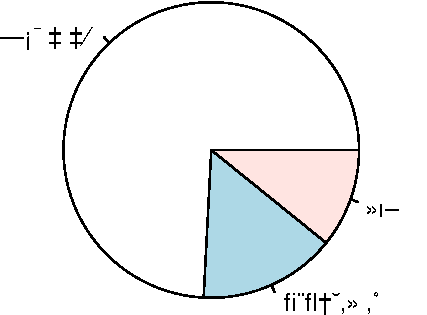
\includegraphics{zzq-detail_files/figure-latex/unnamed-chunk-12-1.pdf}

\subsubsection{泰信优质生活混合}\label{-1}

\begin{longtable}[]{@{}ccccc@{}}
\caption{持仓风格权重分析(\%)}\tabularnewline
\toprule
大盘成长 & 中盘成长 & 小盘成长 & 债券财富指数 & 货币\tabularnewline
\midrule
\endfirsthead
\toprule
大盘成长 & 中盘成长 & 小盘成长 & 债券财富指数 & 货币\tabularnewline
\midrule
\endhead
0.41 & 37 & 41 & 17 & 5\tabularnewline
\bottomrule
\end{longtable}

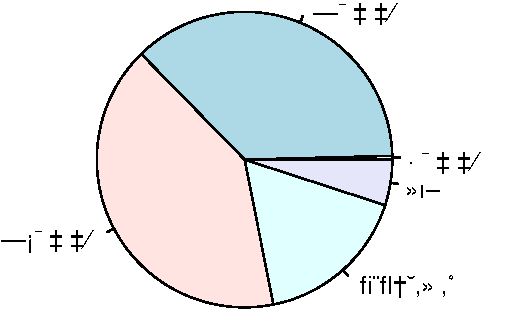
\includegraphics{zzq-detail_files/figure-latex/unnamed-chunk-13-1.pdf}

可见,其重点投资的股票往往都是成长类型的股票。

\subsubsection{泰信先行策略}\label{-1}

\begin{longtable}[]{@{}ccc@{}}
\caption{持仓风格权重分析(\%)}\tabularnewline
\toprule
小盘成长 & 债券财富指数 & 货币\tabularnewline
\midrule
\endfirsthead
\toprule
小盘成长 & 债券财富指数 & 货币\tabularnewline
\midrule
\endhead
57 & 20 & 23\tabularnewline
\bottomrule
\end{longtable}

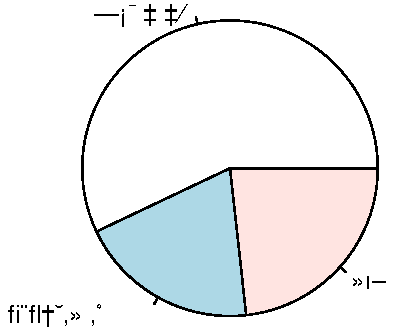
\includegraphics{zzq-detail_files/figure-latex/unnamed-chunk-14-1.pdf}

\subsection{主动风格:偏激进的主动管理}

以其管理的泰信智选成长混合为说明,平均主动管理活跃度为32.5\%,表现为积极的主动管理。在其管理的同期,整个基金行业的同类型基金的主动管理活跃指数为27\%。因此,\emph{对于朱志权的管理风格可以定义为积极的主动管理型。}

另外一只基金泰信优势增长,品均主动管理活跃度为44\%,同期整个基金行业同类型基金主动管理活跃度指数为36\%。\emph{相对来说朱志权呈现了激进的主动管理。}

\section{能力评价}

\subsection{大类资产配置:有效但不稳定}

从下图可以看出,在管理期间朱志权在产品泰信优势增长中将股票仓位控制在50-90\%之间随着股票市场行情而变换,显示除了主动的仓位调节。

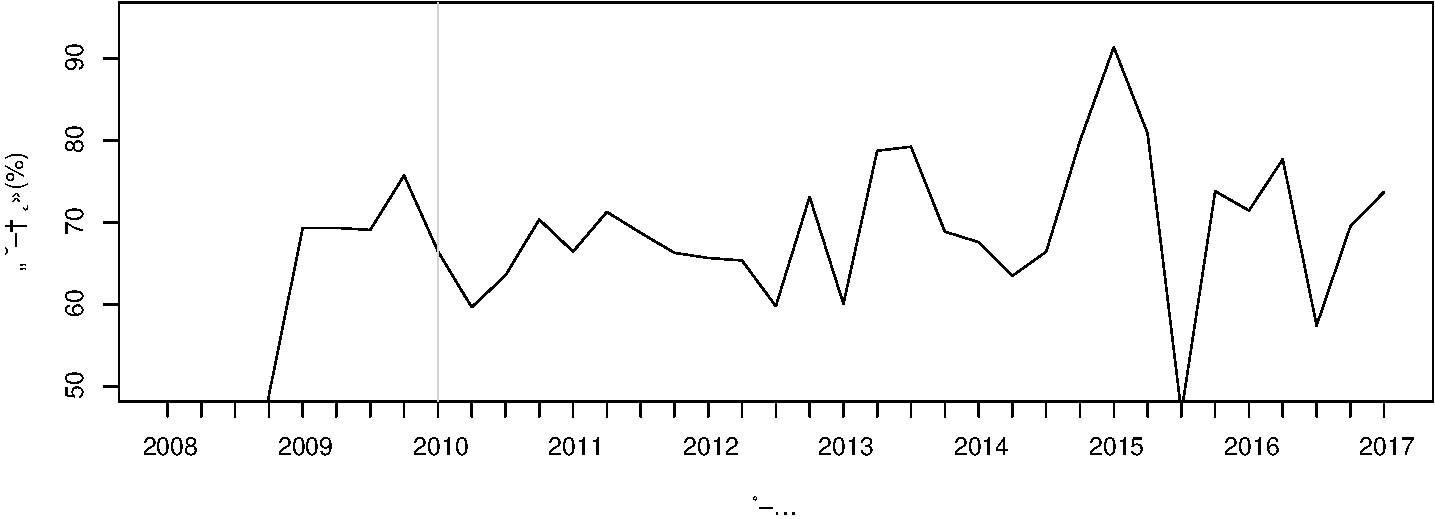
\includegraphics{zzq-detail_files/figure-latex/unnamed-chunk-17-1.pdf}

进一步的计算大类资产配置带来的超额收益。

\subsubsection{泰信优势增长}\label{-1}

\begin{longtable}[]{@{}lc@{}}
\caption{泰信智选成长混合大类资产配置能力统计}\tabularnewline
\toprule
日期 & 大类资产配置超额贡献(\%)\tabularnewline
\midrule
\endfirsthead
\toprule
日期 & 大类资产配置超额贡献(\%)\tabularnewline
\midrule
\endhead
2010 Q1 & -1.5742\tabularnewline
2010 Q2 & -2.1710\tabularnewline
2010 Q3 & 0.7462\tabularnewline
2010 Q4 & 1.6623\tabularnewline
2011 Q1 & 0.3352\tabularnewline
2011 Q2 & -0.6349\tabularnewline
2011 Q3 & -2.0844\tabularnewline
2011 Q4 & -2.2844\tabularnewline
2012 Q1 & 0.5864\tabularnewline
2012 Q2 & -0.4609\tabularnewline
2012 Q3 & 0.0012\tabularnewline
2012 Q4 & 1.1305\tabularnewline
2013 Q1 & -0.4672\tabularnewline
2013 Q2 & -1.8157\tabularnewline
2013 Q3 & 2.8966\tabularnewline
2013 Q4 & 0.4527\tabularnewline
2014 Q1 & -1.7850\tabularnewline
2014 Q2 & -0.9002\tabularnewline
2014 Q3 & 1.0453\tabularnewline
2014 Q4 & 7.2234\tabularnewline
2015 Q1 & 4.3093\tabularnewline
2015 Q2 & 2.3636\tabularnewline
2015 Q3 & -3.0100\tabularnewline
2015 Q4 & -0.0117\tabularnewline
2016 Q1 & -2.7130\tabularnewline
2016 Q2 & -0.3973\tabularnewline
2016 Q3 & -0.1579\tabularnewline
2016 Q4 & 1.0656\tabularnewline
2017 Q1 & 1.0574\tabularnewline
\bottomrule
\end{longtable}

\begin{longtable}[]{@{}cl@{}}
\toprule
平均超额贡献(\%) & 90\%置信区间\tabularnewline
\midrule
\endhead
0.15 & \([-0.38,\infty)\)\tabularnewline
\bottomrule
\end{longtable}

统计显示,在泰信优势增长这支基金的管理上,虽然每季度平均取得
0.15\%的配置收益,但是统计意义上还是不显著。

\subsubsection{泰信优质生活混合}\label{-2}

\begin{longtable}[]{@{}lc@{}}
\caption{泰信智选成长混合大类资产配置能力统计}\tabularnewline
\toprule
日期 & 大类资产配置超额贡献(\%)\tabularnewline
\midrule
\endfirsthead
\toprule
日期 & 大类资产配置超额贡献(\%)\tabularnewline
\midrule
\endhead
2008 Q2 & 0.037\tabularnewline
2008 Q3 & 2.080\tabularnewline
2008 Q4 & 0.089\tabularnewline
2009 Q1 & 3.776\tabularnewline
2009 Q2 & 4.303\tabularnewline
2009 Q3 & -0.658\tabularnewline
2009 Q4 & 2.706\tabularnewline
2010 Q1 & -1.533\tabularnewline
2010 Q2 & -4.561\tabularnewline
2010 Q3 & 2.647\tabularnewline
2010 Q4 & 1.689\tabularnewline
2011 Q1 & 0.479\tabularnewline
2011 Q2 & -1.158\tabularnewline
2011 Q3 & -3.036\tabularnewline
2011 Q4 & -2.624\tabularnewline
2012 Q1 & 0.549\tabularnewline
\bottomrule
\end{longtable}

\begin{longtable}[]{@{}cl@{}}
\toprule
平均超额贡献(\%) & 90\%置信区间\tabularnewline
\midrule
\endhead
0.3 & \([-0.54,\infty)\)\tabularnewline
\bottomrule
\end{longtable}

统计显示,在泰信优质生活混合这支基金的管理上,虽然每季度平均取得0.3\%的配置收益,但是统计意义上还是不显著。

\subsubsection{泰信先行策略}\label{-2}

\begin{longtable}[]{@{}lc@{}}
\caption{泰信智选成长混合大类资产配置能力统计}\tabularnewline
\toprule
日期 & 大类资产配置超额贡献(\%)\tabularnewline
\midrule
\endfirsthead
\toprule
日期 & 大类资产配置超额贡献(\%)\tabularnewline
\midrule
\endhead
2012 Q1 & 0.72\tabularnewline
2012 Q2 & -0.35\tabularnewline
2012 Q3 & -0.45\tabularnewline
2012 Q4 & 0.90\tabularnewline
2013 Q1 & -0.37\tabularnewline
2013 Q2 & -1.96\tabularnewline
2013 Q3 & 2.25\tabularnewline
2013 Q4 & -0.13\tabularnewline
2014 Q1 & -2.63\tabularnewline
2014 Q2 & -0.75\tabularnewline
2014 Q3 & 2.76\tabularnewline
2014 Q4 & 9.07\tabularnewline
2015 Q1 & 2.96\tabularnewline
\bottomrule
\end{longtable}

\begin{longtable}[]{@{}cl@{}}
\toprule
平均超额贡献\% & 90\%置信区间\tabularnewline
\midrule
\endhead
0.92 & \([-0.19,\infty)\)\tabularnewline
\bottomrule
\end{longtable}

统计显示,在泰信先行策略这支基金的管理上,每季度平均取得高达
0.92\%的配置收益,
但是统计意义上并不显著。因此朱志权显示出有效但是不稳定的大类资产配置的能力。

朱志权自己认为判断市场的高点和低点是困难的,但是判断市场具体所处于什么样的阶段是可以的。在这样的判断基础上动态的调整股票整体仓位获取一定程度的配置收益是顺理成章的。同时,也因为不能较好的把握市场的拐点,在市场转变时出现超配或低配进而形成配置损失也难以避免。从整体上看,中国的公募基金管理者,鲜有对于经济规律与走势把握能力强,进而能够获得稳健配置收益的。在这样的前提下,朱志权算是具备相比较的大类资产配置能力的基金经理。

\subsection{行业配置能力:弱}

既然基金产品的超额收益并非得益于大类资产的配置,那么比如来自与行业配置、选股以及择时的能力。需要提前指出的是,这三个能力在逻辑与实践中都不是相互独立的。好的投资标的往往也意味着好的投资时机,而好股票的挖掘与选择自然也带来了相应行业的配置偏好。但是这三种能力又在某种程度上可以区别开来,因为它们毕竟是在投资的不同决策层面和时点上的投资活动。我们认为:

\begin{longtable}[]{@{}lll@{}}
\toprule
行为 & 动机 & 度量方法\tabularnewline
\midrule
\endhead
行业配置 & smart beta & \(\sum(w_i-w_i^B)(r_i^B-r^B)\)\tabularnewline
择股 & 持续的alpha & \(\sum w_{i}(r_{i}^F-r_{i}^B)\)\tabularnewline
择时 & 动态的alpha & 未解释的差额部分\tabularnewline
\bottomrule
\end{longtable}

因为所获得数据精确程度的不同,我们计算的以上三个方面能力对于总超额收益的贡献比例可能是不精确的,读者应该更多的关注其相对值以及相关的统计推论。

\begin{longtable}[]{@{}lcc@{}}
\caption{泰信优势增长行业配置能力}\tabularnewline
\toprule
日期 & 行业配置成功率\% & 行业配置贡献超额收益率\%\tabularnewline
\midrule
\endfirsthead
\toprule
日期 & 行业配置成功率\% & 行业配置贡献超额收益率\%\tabularnewline
\midrule
\endhead
2010 Q1 & 11.1 & 1.13\tabularnewline
2010 Q2 & 12.5 & -3.18\tabularnewline
2010 Q3 & 11.1 & 5.19\tabularnewline
2010 Q4 & 10.0 & 1.45\tabularnewline
2011 Q1 & 10.0 & -2.35\tabularnewline
2011 Q2 & -11.1 & -1.81\tabularnewline
2011 Q3 & 7.1 & 7.59\tabularnewline
2011 Q4 & 7.7 & -1.40\tabularnewline
2012 Q1 & -7.1 & -16.51\tabularnewline
2012 Q2 & 7.1 & 6.60\tabularnewline
2012 Q3 & -9.1 & 0.02\tabularnewline
2012 Q4 & 6.7 & -4.83\tabularnewline
2013 Q1 & -8.3 & 2.65\tabularnewline
2013 Q2 & 12.5 & 5.49\tabularnewline
2013 Q3 & 10.0 & 13.14\tabularnewline
2013 Q4 & 11.1 & -2.50\tabularnewline
2014 Q1 & 12.5 & 2.60\tabularnewline
2014 Q2 & 12.5 & 3.03\tabularnewline
2014 Q3 & 10.0 & 0.91\tabularnewline
2014 Q4 & 10.0 & -17.89\tabularnewline
2015 Q1 & 14.3 & 15.41\tabularnewline
2015 Q2 & 11.1 & 4.70\tabularnewline
2015 Q4 & 10.0 & 7.73\tabularnewline
2016 Q1 & -10.0 & -4.12\tabularnewline
2016 Q2 & 9.1 & -0.32\tabularnewline
2016 Q4 & -9.1 & -2.24\tabularnewline
2017 Q1 & 9.1 & -2.75\tabularnewline
\bottomrule
\end{longtable}

\begin{longtable}[]{@{}cl@{}}
\toprule
平均超额贡献\% & 90\%置信区间\tabularnewline
\midrule
\endhead
0.66 & \([-1.16,\infty)\)\tabularnewline
\bottomrule
\end{longtable}

从统计结果可以看出,朱志权在泰信优势增长基金的管理上没有显示突出的行业配置能力,平均超额表现为0.66\%每半年,年化2.66\%,但是统计上并不显著。

\begin{longtable}[]{@{}lcc@{}}
\caption{泰信优质生活混合行业配置能力}\tabularnewline
\toprule
日期 & 行业配置成功率\% & 行业配置贡献超额收益率\%\tabularnewline
\midrule
\endfirsthead
\toprule
日期 & 行业配置成功率\% & 行业配置贡献超额收益率\%\tabularnewline
\midrule
\endhead
2010 Q1 & -10.0 & 1.2\tabularnewline
2010 Q2 & -10.0 & -4.3\tabularnewline
2010 Q3 & -10.0 & 4.9\tabularnewline
2010 Q4 & -10.0 & 3.2\tabularnewline
2011 Q1 & 11.1 & -2.4\tabularnewline
2011 Q2 & -11.1 & -3.5\tabularnewline
2011 Q3 & 6.7 & 9.1\tabularnewline
2011 Q4 & 7.1 & 3.4\tabularnewline
2012 Q1 & -5.9 & -15.2\tabularnewline
\bottomrule
\end{longtable}

\begin{longtable}[]{@{}cl@{}}
\toprule
平均超额贡献\% & 90\%置信区间\tabularnewline
\midrule
\endhead
-0.41 & \([-3.69,\infty)\)\tabularnewline
\bottomrule
\end{longtable}

从统计结果可以看出,朱志权在泰信优质生活混合基金的管理上没有体现出行业配置能力,平均超额表现为-0.41\%每半年,年化-1.64\%。

\begin{longtable}[]{@{}lcc@{}}
\caption{泰信先行策略行业配置能力}\tabularnewline
\toprule
日期 & 行业配置成功率\% & 行业配置贡献超额收益率\%\tabularnewline
\midrule
\endfirsthead
\toprule
日期 & 行业配置成功率\% & 行业配置贡献超额收益率\%\tabularnewline
\midrule
\endhead
2012 Q1 & -5.9 & -14.36\tabularnewline
2012 Q2 & 6.2 & 7.88\tabularnewline
2012 Q3 & -7.1 & -0.53\tabularnewline
2012 Q4 & 6.7 & -4.22\tabularnewline
2013 Q1 & -7.7 & 2.38\tabularnewline
2013 Q2 & -7.1 & 5.62\tabularnewline
2013 Q3 & 7.1 & 10.02\tabularnewline
2013 Q4 & -7.7 & -1.37\tabularnewline
2014 Q1 & 8.3 & 1.47\tabularnewline
2014 Q2 & 10.0 & 2.30\tabularnewline
2014 Q3 & -8.3 & 1.42\tabularnewline
2014 Q4 & 6.2 & -22.05\tabularnewline
2015 Q1 & 10.0 & 22.40\tabularnewline
\bottomrule
\end{longtable}

\begin{longtable}[]{@{}cl@{}}
\toprule
平均超额贡献\% & 90\%置信区间\tabularnewline
\midrule
\endhead
0.84 & \([-3.24,\infty)\)\tabularnewline
\bottomrule
\end{longtable}

从统计结果可以看出,朱志权在泰信先行策略基金的管理上显示了一定的行业配置能力,平均超额表现为0.84\%每半年,年化3.42\%。但是波动较大,统计不显著。最主要的失误是2014底对于券商行业的业绩表现判断失误。

\subsection{择股能力:高亮明星的下坡路}

公开渠道获得的持仓数据频率为每半年一次。我们依据此数据分析基金管理人的择股能力。当然,由于更新频率粗糙,读者有理由担心计算精度的问题。不过从另外一个角度看,我们所谓的择股能力是对照于择时能力而言获取相对持续的alpha的能力。这里的相对持续,完全可以根据我们研究的需要而定义。此处,定义半年为一个相对持续的alpha的标准,也是合情合理的。当前受制于数据不完整,此项能力分析最早只能回溯到2013年。

\begin{longtable}[]{@{}lcc@{}}
\caption{泰信优势增长择股能力}\tabularnewline
\toprule
日期 & 行业择股成功率\% & 择股贡献超额收益率\%\tabularnewline
\midrule
\endfirsthead
\toprule
日期 & 行业择股成功率\% & 择股贡献超额收益率\%\tabularnewline
\midrule
\endhead
2013 Q1-2 & -9.1 & 31.2\tabularnewline
2013 Q3-4 & 11.1 & 16.1\tabularnewline
2014 Q1-2 & 11.1 & 7.8\tabularnewline
2014 Q3-4 & 7.7 & 10.6\tabularnewline
2015 Q1-2 & 9.1 & 53.9\tabularnewline
2015 Q3-4 & 9.1 & 6.4\tabularnewline
2016 Q1-2 & -8.3 & -2.9\tabularnewline
2016 Q3-4 & -8.3 & -10.2\tabularnewline
2017 Q1-2 & 9.1 & -3.6\tabularnewline
2017 Q3-4 & 16.7 & -0.9\tabularnewline
\bottomrule
\end{longtable}

\begin{longtable}[]{@{}cl@{}}
\toprule
平均超额贡献\% & 90\%置信区间\tabularnewline
\midrule
\endhead
11 & \([2.46,\infty)\)\tabularnewline
\bottomrule
\end{longtable}

从统计结果可以看出,朱志权在泰信优势增长基金的管理上显示了明显的择股能力------即他能够选择出在未来6个月的投资周期上回报好于对应行业指数表现的股票组合,而且择股能力贡献的平均超额表现高达10.85\%每半年,年化22.88\%。

\begin{longtable}[]{@{}lcc@{}}
\caption{泰信先行策略择股能力}\tabularnewline
\toprule
日期 & 行业择股成功率\% & 择股贡献超额收益率\%\tabularnewline
\midrule
\endfirsthead
\toprule
日期 & 行业择股成功率\% & 择股贡献超额收益率\%\tabularnewline
\midrule
\endhead
2013 Q1-2 & -6.7 & 23.9\tabularnewline
2013 Q3-4 & 6.7 & 7.6\tabularnewline
2014 Q1-2 & 7.7 & -1.2\tabularnewline
2014 Q3-4 & -5.9 & 4.4\tabularnewline
2015 Q1-2 & 6.2 & 76.0\tabularnewline
\bottomrule
\end{longtable}

\begin{longtable}[]{@{}cl@{}}
\toprule
平均超额贡献\% & 90\%置信区间\tabularnewline
\midrule
\endhead
22 & \([0.54,\infty)\)\tabularnewline
\bottomrule
\end{longtable}

从统计结果可以看出,朱志权在泰信先行策略基金的管理上显示了明显的择股能力------即他能够选择出在未来6个月的投资周期上回报好于对应行业指数表现的股票组合,而且择股能力贡献的平均超额表现高达22.15\%每半年,年化49.22\%。须知这是在沪深300成长指数成分股和备选股中选择的股票,能够有这样的表现实属不易。

当然,我们也需要客观的指出,朱志权的超强的择股能力的一部分贡献,来自与2015年上半年。尽管我们在计算择股能力的时候,使用的是超额收益,即减去参照指标(一般是沪深300指数)后的超出部分。按理已经排除了牛市的影响,将其完全归集为择股能力并无问题。但是需要指出,中国市场的问题很多,尤其牛市期间,``妖股''频出。这些不可言状的``妖股'',也许成就了基金经理人的辉煌人生,不无不可,毕竟``人脉''或者``运气''也是能力的一部分。但就以此建立一个择股能力的最高标杆,则误导大众了。因此可以考虑将这段时间的数据排除出去进行分析。那样的话,我们得出朱志权的择股能力也是比较强的(当然,不再是超强)。

\subsection{择时能力:灾难性}

择时能力在本文的设定中包括以下方面:

\begin{itemize}
\tightlist
\item
  交易周期短于半年的动态alpha机会,如一些短期事件性投资机会、相对明确的业绩反转预期等。
\item
  上升通道中的止盈能力
\item
  下降通道中的止亏能力
\end{itemize}

所以择时能力并不总是能够带来正的超额收益,但是它能够确保落袋为安(止盈能力)或者保命再战(止亏能力),对于提高基金的风险收益比(如夏普率)是十分重要的。

\begin{longtable}[]{@{}lc@{}}
\caption{泰信优势增长择时能力}\tabularnewline
\toprule
日期 & 择时能力贡献超额收益率\%\tabularnewline
\midrule
\endfirsthead
\toprule
日期 & 择时能力贡献超额收益率\%\tabularnewline
\midrule
\endhead
2013 Q1-2 & -12.0\tabularnewline
2013 Q3-4 & 3.9\tabularnewline
2014 Q1-2 & 2.6\tabularnewline
2014 Q3-4 & -12.1\tabularnewline
2015 Q1-2 & -26.3\tabularnewline
2015 Q3-4 & -9.0\tabularnewline
2016 Q1-2 & -10.3\tabularnewline
2016 Q3-4 & -3.0\tabularnewline
2017 Q1-2 & 1.9\tabularnewline
\bottomrule
\end{longtable}

\begin{longtable}[]{@{}cl@{}}
\toprule
平均超额贡献\% & 90\%置信区间\tabularnewline
\midrule
\endhead
-7.1 & \([-11.64,\infty)\)\tabularnewline
\bottomrule
\end{longtable}

从上表中可以看出,朱志权在泰信优势增长基金的管理上显示了明显的负的择时能力,而且择时能力贡献的平均超额表现多达-7.14\%每半年,年化-13.78\%。

\begin{longtable}[]{@{}lc@{}}
\caption{泰信先行策略择时能力}\tabularnewline
\toprule
日期 & 择时能力贡献超额收益率\%\tabularnewline
\midrule
\endfirsthead
\toprule
日期 & 择时能力贡献超额收益率\%\tabularnewline
\midrule
\endhead
2013 Q1-2 & -10.2\tabularnewline
2013 Q3-4 & 0.4\tabularnewline
2014 Q1-2 & -2.2\tabularnewline
2014 Q3-4 & -9.7\tabularnewline
2015 Q1-2 & -59.3\tabularnewline
\bottomrule
\end{longtable}

\begin{longtable}[]{@{}cl@{}}
\toprule
平均超额贡献\% & 90\%置信区间\tabularnewline
\midrule
\endhead
-16 & \([-33.01,\infty)\)\tabularnewline
\bottomrule
\end{longtable}

从上表中可以看出,朱志权在泰信先行策略基金的管理上显示了明显的负的择时能力,而且择时能力贡献的平均超额表现多达-16.19\%每半年,年化-29.76\%。

综上,我们认为朱志权作为一名低换手的坚定的成长股投资者,他在择时能力上的灾难性的表现,部分可以归结为其止赢能力上的欠缺。

\section{投资方法体系}

\subsection{成长性}

关于成长股,虽然当前不是成长股的收获周期,但是却是投资成长股的好时机。在市场风险偏好降低的时候,水落石出,自然的筛选了优秀的成长股。选择成长股:

\begin{itemize}
\tightlist
\item
  关注于未来2-3年能成长的公司,也就是要具备一定安全边际或者确定性的成长。
\item
  关注于行业模式,尤其是已经验证了的行业模式。比如苹果产业链中的企业,如果已近在一个细分领域内做到全行业第一的,估值往往在100亿左右。因为电子产业的相关性,其必然可以相对容易的扩展,发展新的细分领域,若有2个以上产品成为行业第一,则可以有200-400亿元的市值,如果继续往下发展,成为平台型的企业则可能有千亿以上的市值。其背后的逻辑的产业的相似性为成功企业复制管理经验、扩展供应链以及品牌延伸提供了便捷。
\item
  投资成长股最重要的是选对行业,看行业发展的势头,其次才是看企业,甚至可以在看好的行业内打一个分散的包作为投资组合。
\end{itemize}

\subsubsection{成长股的PE之辨}\label{pe}

有投资者认为成长股也要关注PE,控制估值。如国泰基金的申坤。但是朱志权认为成长股如果PE低,说明它的业绩已经到达最高峰,成长性消失,此时投资只能收获市场波动的收益。真正投资成长股,要冲着营业输入翻翻,收入翻翻的企业去,这样的企业即便在市场低迷的时候也不是低PE的。

\subsubsection{成长股的投资时机}

前提是一定要在研究范围内长期的跟踪,时点选择上可以:

\begin{itemize}
\tightlist
\item
  在市场都不关注的时候提前买有特色的成长股
\item
  在第一根阳线的时候买
\end{itemize}

\subsubsection{看好和擅长的投资方向}

当前看好两个投资方向:

\begin{enumerate}
\def\labelenumi{\arabic{enumi}.}
\tightlist
\item
  苹果产业链
\item
  特斯拉产业链
\item
  医疗服务
\end{enumerate}

\subsection{风险控制方法}

\begin{enumerate}
\def\labelenumi{\arabic{enumi}.}
\tightlist
\item
  相对分散、阶段集中
\item
  作为基金经理1/3投资于长期持有的成长股作为底仓,1/3投资于一年左右机会的股票获得波动收益,1/3投资于短期博弈机会。
\end{enumerate}

\section{评价}

朱志权是既往的成长股明星,在市场风格转变之后,经历了一段修养身心的蛰伏。我们基于公开信息,进行深度的科学分析,结合与其面对面的交流,做出如下评判:

\begin{enumerate}
\def\labelenumi{\arabic{enumi}.}
\tightlist
\item
  他是有着丰富投资经验的坚定的、专注的成长股投资者;
\item
  他是低换手、高PE偏激进的主动型投资者;
\item
  他在成长股的选择上有较强的判断能力,对于行业、企业的成长方向有很强的把握能力;
\item
  他具备一定的大类资产配置能力,这主要表现在对于股票市场所处周期有一定的判断能力,但是对于市场拐点没有预测能力。同时对于全市场的行业前景没有大局的判断能力,表现在行业配置能力较弱。
\item
  他不具备择时能力,尤其不善于止赢。
\end{enumerate}

\end{document}
